\documentclass[10.5pt,a4paper,dvipdfmx]{jsarticle}
% \documentclass[10.5pt,a4paper,dvipdfmx]{jsarticle}
% 画像
\usepackage[dvipdfmx]{graphicx}
% 表
\usepackage{booktabs}
% 数式
\usepackage{amsmath}
% ベクトル
\usepackage{bm}
\usepackage{tcolorbox}

\usepackage{siunitx}
% コード
\usepackage{listings,jvlisting}
% コードの色
\usepackage{color}
\definecolor{OliveGreen}{rgb}{0.0,0.6,0.0}
\definecolor{Orenge}{rgb}{0.89,0.55,0}
\definecolor{SkyBlue}{rgb}{0.28,0.28,0.95}
% ここからコードの表示に関する設定
\lstset{
  language=C,
  basicstyle={\ttfamily},
  identifierstyle={\small},
  commentstyle={\small\itshape},
  keywordstyle={\small\bfseries},
  ndkeywordstyle={\small},
  stringstyle={\small\ttfamily},
  frame={tb},
  breaklines=true,
  columns=[l]{fullflexible},
  numbers=left,
  xrightmargin=0zw,
  xleftmargin=3zw,
  numberstyle={\scriptsize},
  stepnumber=1,
  numbersep=1zw,
  lineskip=-0.5ex,
  keepspaces=true,
  keywordstyle={\color{SkyBlue}},
  commentstyle={\color{OliveGreen}},
  stringstyle=\color{Orenge},
  showstringspaces=false
}
\renewcommand{\lstlistingname}{Code}
\NewDocumentCommand{\codeword}{v}{%
    \texttt{\textcolor{blue}{#1}}%  
}
% リンク
\usepackage[dvipdfmx]{hyperref}

\title{前期実験 I3実験 レポート}
\author{18班 古谷優人 \\ 共同実験者  福島 幸弥}
\date{\today}


\begin{document}

\maketitle

\section{概要}
I2実験\cite{link}で作成したコードをもとに, いくつかの機能を追加したコードを実装した. (リンク:\url{https://github.com/furuSchool/experiment_I3})

実装した機能と, 工夫した点, 改善できる点などを以下に述べる. 
また, 作成を試みたが, 失敗に終わったものも同時にあげた. 

\section{実装した機能}
I2 実験まででは, 双方向に電話ができるプログラムを作成したが, その機能に追加して, テキストの送信やファイルの送信などが自由にできるようなプログラムを作成しようと考え, 実装を行った. 

詳しくは後に述べるが, 始めはサーバー側が二つ以上ポートを開くことにより実装しようとしたがうまく動作しなかったため, 一つのポートを用いて, 入力によってモードを変更することで, 音声以外のやりとりも可能となるように実装を行った. 

また, 他にも様々な機能を作成した. 

\vskip\baselineskip

\subsection{発信音}
電話機能の使用感を実際の電話のものに近づける手段として,発着信音の追加を試みた.

コードの一部をCode~\ref{code:ringtone}に示す.

\begin{lstlisting}[caption=ring tone, label=code:ringtone]
void *play_sound(void *arg) {
    while (1) {
        if(system("play phone.wav --no-show-progress 2>/dev/null") != 0) {
            perror("system");
            exit(1);
        };
    }
    return NULL;
}

int flags = fcntl(ss, F_GETFL, 0);
fcntl(ss, F_SETFL, flags | O_NONBLOCK);

struct sockaddr_in client_addr;
socklen_t len = sizeof(struct sockaddr_in);
int s;

pthread_t tid;
if (pthread_create(&tid, NULL, play_sound, NULL) != 0) {
    perror("pthread_create");
    exit(1);
}

while (1) {
    fd_set readfds;
    FD_ZERO(&readfds);
    FD_SET(ss, &readfds);

    struct timeval tv;
    tv.tv_sec = 0;
    tv.tv_usec = 100000; // 0.1 sec

    int activity = select(ss + 1, &readfds, NULL, NULL, &tv);

    if (activity < 0) {
        perror("select");
        exit(1);
    }

    if (FD_ISSET(ss, &readfds)) {
        s = accept(ss, (struct sockaddr *)&client_addr, &len);
        if (s == -1) {
            perror("accept");
        } else {
            printf("Connection Succeeded!\n");
            break;
        }
    }
}

pthread_cancel(tid);
pthread_join(tid, NULL);
\end{lstlisting}
ここでは,select関数を用いて,クライアントの接続を監視している.その間,pthread関数で作成した別スレッドで,system関数を呼び出し続け,phone.wav(フリーの音源サイト\cite{phone.wav}からダウンロードしたもの)を再生している.acceptされると,pthreadはキャンセルされてphone.wavは再生を停止する.

\vskip\baselineskip

ただし, この実装を行うと, 後に述べる file mode の際, クライアントからサーバーにファイルを送信しようとすると, \codeword{recv: Resource temporarily unavailable}というエラーがクライアント側に生じるようになってしまった. そのため, クライアント側からファイルを送信したい場合は, I2 実験時のコードを用いれば良い. 

\vskip\baselineskip

\subsection{モードの切り替え}
まず, 各機能を切り替えるために, モードの切り替えを実装した. コードの一部を, Code \ref{code:mode} に示す. 

\begin{lstlisting}[caption=change mode, label=code:mode]
int isAllTs(const unsigned char *input){
    int length = strlen(input);
    if (length < 1){
        return 0;
    }
    for (int i = 0; i < 10; i++){
        if (input[i] != 'T'){
            return 0;
        }
    }
    return 1;
}

// -- モード変更を行う側 --
char *all_Ts = (char *)malloc((N) * sizeof(char));
memset(all_Ts, 'T', 100);
if (strcmp(input_tmp, "hoge") == 0){
    if (mode != 1){
        mode = 1;
        send(s, all_Ts, N, 0);
        printf("mode is text\n");
    }
}

// -- モード変更をされた側 --
listen_n = recv(s, listen, N, 0);
if (isAllTs(listen)){
    mode = 1;
    printf("mode is changed to text\n");
}
\end{lstlisting}

このように, モード変更を行う側は標準入力を\codeword{input_tmp}にいれ, それが特定の文字列と一致するときに特定の文字を100バイトほど送信し, モードを切り替える. 

一方でモード変更をされた側は, モードを切り替えたことを検知してモードを変更する必要があるため, \codeword{isAllTs()} を用いて, 受け取った文字列が特定の文字の列である場合に, モードを変更する実装を行っている. 

そして, このコードをモードの数だけ実装することで, モードの移行を実現している. 

\vskip\baselineskip

\subsection{電話機能}
まずは, 機能の基本として電話を実装している. コードは, I2実験で実装したものとほとんど同じである. 

変更点としては, 以下の通りである. 標準入力が見やすいように, \codeword{rec,play} のオプションに \codeword{--no-show-progress, 2>/dev/null} を追加して, ログが標準出力されないようにした. 

また, テキストのやり取り中など音声の録音が必要のない場面でも, 録音を続け, 必要のない音声データを捨てるようなプログラムになっており, 少し無駄が生じている. 

\vskip\baselineskip

\subsection{テキスト送受信機能}
標準入力に特定の文字列を入力することで, テキストの送受信ができるモードを実装した. Code \ref{code:text} に, そのコードの一部を示す. 

\begin{lstlisting}[caption=text mode, label=code:text]
fd_set readfds, writefds;
FD_ZERO(&readfds);
FD_SET(STDIN_FILENO, &readfds);
FD_SET(s, &readfds);
FD_ZERO(&writefds);
FD_SET(s, &writefds);
// -- 中略 --
// mode = 1 が text mode
else if (mode == 1){
    int ret = select(maxfd + 1, &readfds, &writefds, NULL, NULL);
    if (FD_ISSET(s, &readfds)){
        unsigned char read_text[N];
        int read_n = recv(s, read_text, N, 0);
        if (read_n == -1){
            perror("recv");
            exit(1);
        }
        if (read_n == 0)
            break;
        if (isAllAs(read_text)){
            mode = 0;
            printf("mode is changed to audio\n");
        }
        else if (isAllFs(read_text)){
            mode = 3;
            printf("mode is changed to receive file\n");
        }
        else{
            printf("received message: ");
            fwrite(read_text, sizeof(unsigned char), read_n, stdout);
        }
    }
}
// -- 中略 --
if (FD_ISSET(STDIN_FILENO, &readfds)){
    n = read(0, input, N);
    //  -- 中略 --
    // 標準入力が mode 変更文字でないかを確認した後, mode = 1 であれば 標準入力を送信している.
    else if (mode == 1){
        send(s, input, N, 0);
        printf("send complete!: %s", input);
    }
    // -- 中略 --
}
\end{lstlisting}

このように, \codeword{select} を用いて, 標準入力が入力された場合に mode 変更に関わる文字でないかを判定し, さらに text mode である時のみ, その値を相手に送信している. 

そして, メッセージを受け取る側は, 受け取ったソケットの中身を標準出力している. ただし, その値が特定の文字列であれば標準出力をせずにモードの変更を行う必要があるため, その判定も同時に行なっている. 

その他工夫した点として, モード変更をする側とされる側にはタイムラグがあるため, 例えば, 電話から text mode に変更中, 送信された音声がテキストと解釈され, 標準出力されるようなことがあったため, Code\ref{code:text_time}  のようなコードを実装することで, 相手側のモードが変更される前にモードを変更してしまうことを防いだ. 
\begin{lstlisting}[caption=time handle, label=code:text_time]
send(s, all_Ts, N, 0);

fd_set tmp_readfds;
struct timeval timeout;
int retval;
while (1){
    FD_ZERO(&tmp_readfds);
    FD_SET(s, &tmp_readfds);
    timeout.tv_sec = 1;
    timeout.tv_usec = 0;
    retval = select(s + 1, &tmp_readfds, NULL, NULL, &timeout);
    if (retval){
        recv(s, buffer, sizeof(buffer), 0);
    }
    else{
        break;
    }
}
printf("mode is text\n");
\end{lstlisting}
ここでは, モードの変更命令を相手側に送信した後, 少し時間を置くことでモードの変更猶予を与えている. 

\vskip\baselineskip

\subsection{ファイル送受信機能}
電話とFAXの機能を両立することを目指して, ファイルの送受信を実装した. ファイルを送信する側と受信する側ではコードが異なるため, 送信する側を Code5 に, 受信する側を Code 6 にそれぞれ示す.

\begin{lstlisting}[caption=file sending]
FILE *fp = fopen(input_tmp, "r");
// -- 中略 --(モードの変更を検知するコード)
if (fp == NULL){
    perror("fopen");
}else{
    int read_filename_n;
    while ((read_filename_n = fread(buffer, 1, N, fp)) > 0)
    {
        if (send(s, buffer, read_filename_n, 0) == -1){
            perror("Error send data");
            fclose(fp);
            exit(1);
        }
    }
    printf("Send: %s!\n", input_tmp);
    send(s, all_Ks, N, 0);
    mode = 0;
    printf("mode is changed to audio\n");
}
\end{lstlisting}

\begin{lstlisting}[caption=file receiving]
printf("preparing to receive file\n");
time_t t = time(NULL);
struct tm *tm_info = localtime(&t);
char filename[256];
strftime(filename, sizeof(filename), "sended_file_%Y-%m-%d_%H-%M-%S.txt", tm_info);
FILE *sended_fp = fopen(filename, "a");
int read_filename_n;
while (1){
    unsigned char read_text[N];
    int read_n = recv(s, read_text, N, 0);
    if (read_n == 0)
        break;
    if (isAllAs(read_text)){
        mode = 0;
        printf("file sending is canceled\n");
        printf("mode is changed to audio\n");
        break;
    }else if (isAllKs(read_text)){
        mode = 0;
        printf("Received file!\n");
        printf("mode is changed to audio\n");
        break;
    } else if (fwrite(read_text, sizeof(unsigned char), read_n, sended_fp) != read_n){
        perror("fwrite");
        exit(1);
    }
}
fclose(sended_fp);
\end{lstlisting}


Code 5 では, まず, 標準入力から, 送信したいファイル名を受け取り,ファイルが存在しない場合はエラーを出力する. 次に, ファイルが存在する場合は, ファイルの内容を読み, 全てソケットを用いて相手側に送信する. 

そして, ファイルの読み取りが終了したら, 特定の文字列を送信することで, モード変更を伝え, 基本のモードである電話に戻っている. なお, 標準入力からファイル名を読み取る前に, モードの変更を示す文字列かを判断しているが, ここでは省略している. 

\vskip\baselineskip

一方, Code 6 では, まず現在の時間を取得して, "sended\_file\_2000-01-01\_01-01-01.txt" のようなファイルを作成する. そして, 受け取ったソケットを読み取り, まずはモード変換命令でないかどうかを判断する. もし, モード変換命令でない場合は, ひたすら受け取ったソケットの内容を作成したファイルに書き込む. 

\vskip\baselineskip

このような二つのコードを組み合わせることで, FAX のようにファイルを送受信することができるプログラムの作成を行った. 

\vskip\baselineskip

この機能の問題点として, モード変更をされた側がうまくモード変更命令を受け取れず, モードが変更できないことがあった. 同じPC間では問題はあまり生じなかったが, 異なるPC間ではその問題が顕著になり, うまく file mode を終了できないことがあった. 

この原因として, ファイルを送信したすぐ後にモード変更命令を送信しているため, ファイルの内容とモード変更命令を分けられていない可能性があった.
そこで, ファイルの送信とモード変更命令の間を1秒間ほどあけることで, ファイルの内容とモード変更命令を区別できるよう工夫を行い, 機能を実現させた.

\vskip\baselineskip

\subsection{ミュート機能}
通話のミュート機能を実装した. これを流用して,通話から退出できる機能も同時に追加した.
Code \ref{code:mute} に, そのコードの一部を示す. 

\begin{lstlisting}[caption=file receiving, label=code:mute]
if (FD_ISSET(STDIN_FILENO, &readfds)){
// -- 中略 --
    if (strcmp(input_tmp, "1") == 0 || strcmp(input_tmp, "text") == 0){
    // -- 中略 --
    }
    // -- 中略 --
    else if (mode == 0 && strcmp(input_tmp, "m") == 0){
        if (mute_mode) {
            printf("Already mute mode\n");
        }
        else {
            mute_mode = 1;
            printf("Moved to mute mode\n");
        }
    }
    else if (strcmp(input_tmp, "s") == 0) {
        if (mute_mode) {
            mute_mode = 0;
            printf("Moved to speaker mode\n");
        }
        else {
            printf("Already speaker mode\n");
        }
    }
    else if (strcmp(input_tmp, "q") == 0) break;
    else{
        printf("invalid command: %s", input);
    }
}
\end{lstlisting}
Code \ref{code:mute}では, "m" をミュート命令, "s" をミュート解除命令, "q" を退室命令として, 標準入力から判断している. 相手が"ミュート・退室した"というのも, モード変更と同様に伝達できると考えられるが, 時間の関係で実装はできなかった. 

加えて, 電話機能に戻った時は, 前の状態に関わらずミュートにならないように, すなわち \codeword{mute\_mode = 0} となるようにした. 

\vskip\baselineskip

\subsection{実際の出力例}
実際に機能を実行したコマンドラインの結果の例を図\ref{fig:server}, \ref{fig:client}に示す.

\begin{figure}[tb]
  \begin{minipage}[c]{0.5\hsize}
    \centering
    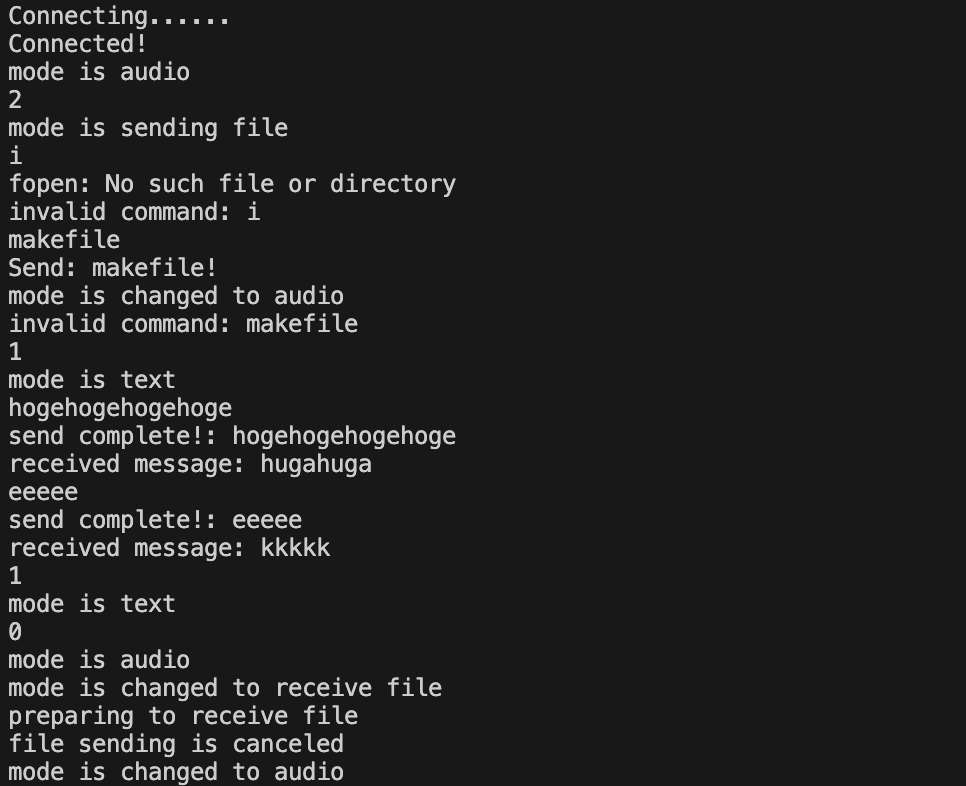
\includegraphics[keepaspectratio,width=0.9
    \columnwidth]{fig/server.png}
    \caption{サーバー側のコマンドライン}
    \label{fig:server}
  \end{minipage}
  \begin{minipage}[c]{0.5\hsize}
    \centering
    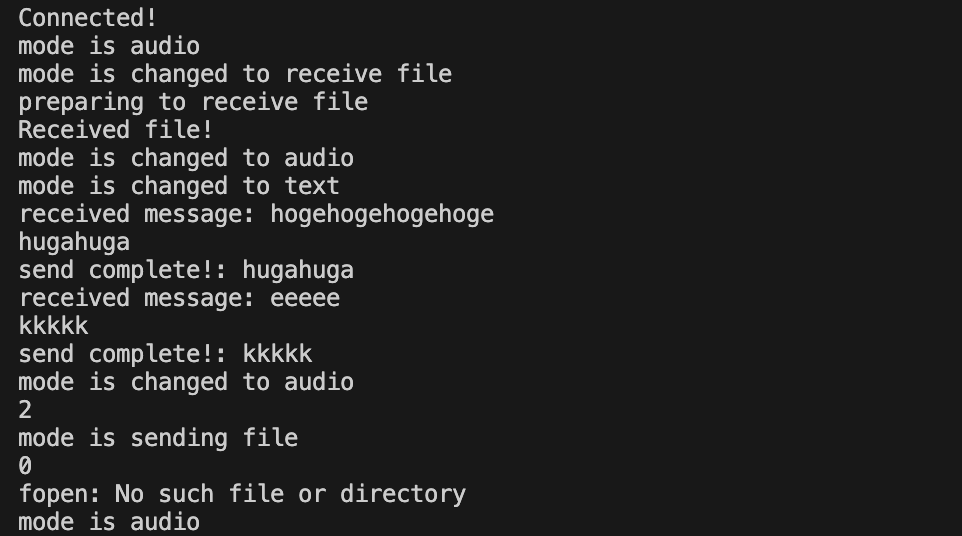
\includegraphics[keepaspectratio,width=0.9
    \columnwidth]{fig/client.png}
    \caption{クライアント側のコマンドライン}
    \label{fig:client}
  \end{minipage}
\end{figure}

なお, ここでは, "0"が audio mode に変更, "1"が text mode に変更, "2"が file mode に変更するための標準入力となっている. 

サーバー側を A, クライアント側を B として, やりとりを説明する. 

まず, A が "2"を入力して file mode に変更し, それが B に知らせられる.  一度, ファイル名・モード変更として適切でない "i"を入力し, エラーが生じた後, 同じディレクトリ内にある"makefile"を選択し, ファイルを送信した. Bでは, 受信したファイルが同じディレクトリ内に"sended\_file\_2000-01-01\_01-01-01.txt"として保存された. 

次に, A が "1" を入力して text mode に変更し, それが B に知らせられる. A と B で text のやりとりを行った後, A が "0" を入力して audio mode に変更し, それが B に知らされる. 

最後に, B が "2"を入力して file mode に変更し, それが A に知らされたものの, B は "0" を入力してファイルの送信をキャンセルし, audio mode に変更した. 

\vskip\baselineskip

\subsection{その他}
\begin{enumerate}
    \item コードを作成するにあたり分割コンパイルを行い, ソケットの作成, 会話中の動作などは, 関数を利用して main のファイルとは別の場所に格納した. 

    \item 音声のデータを使わないときに, リフレッシュを行わないと, 前のデータが残ってしまい, 音声のやりとりに大きなタイムラグが生じることがあったため, 下記のコードをいれ, 音声データが残らないようにした. 
    
    \codeword{fread(buffer, 1, sizeof(buffer), fp_rec);fread(buffer, 1, sizeof(buffer), fp_play);}
\end{enumerate}

\vskip\baselineskip

\section{実装できなかった機能}
\subsection{ボイスチェンジ機能}
I1実験にて作成した, ボイスチェンジャーを用いて, 電話する際にボイスチェンジ機能を実現し, モードの一つとして実装しようと試みた. 

しかし, ボイスチェンジした後にうまく音声が再生されない, 再生されたとしてもデータの切れ目で音が鳴る, ピッチが変更されないなどの問題が生じ, 原因が特定できず実装できなかった. 

データの切れ目で音が鳴るのは, データをつぎはぎしているためと考えられ, 実際, 遅延の増大を無視して一度にボイスチェンジするデータ量を減らすと, 気にならなくなった. 三角窓関数を用いて除去しようと試みたが失敗に終わった. 

\vskip\baselineskip

\subsection{音声・チャット同時対応}
サーバー側がポートを二つ以上開くことで, 音声のやりとりと文章のやりとりを同時に行うような実装を考えた. 具体的なコードを Code\ref{code:port_server},  \ref{code:port_client}に示す.
なお, エラーハンドリングは省略している. 

\begin{lstlisting}[caption=音声・チャット同時対応(サーバー側), label=code:port_server]
// audio
int ss = socket(PF_INET, SOCK_STREAM, 0);
struct sockaddr_in addr;
addr.sin_family = AF_INET;
addr.sin_addr.s_addr = INADDR_ANY;
addr.sin_port = htons(port_number);
int bind_error = bind(ss, (struct sockaddr *)&addr, sizeof(addr));

listen(ss, 10)

struct sockaddr_in client_addr;
socklen_t len = sizeof(struct sockaddr_in);
int s = accept(ss, (struct sockaddr *)&client_addr, &len);

// text
int text_ss = socket(PF_INET, SOCK_STREAM, 0);
struct sockaddr_in text_addr;
text_addr.sin_family = AF_INET;
text_addr.sin_addr.s_addr = INADDR_ANY;
text_addr.sin_port = htons(port_number + 10);
bind_error = bind(text_ss, (struct sockaddr *)&text_addr, sizeof(text_addr));

listen(text_ss, 10)

struct sockaddr_in client_text_addr;
socklen_t text_len = sizeof(struct sockaddr_in);
int text_sock = accept(text_ss, (struct sockaddr *)&client_text_addr, &text_len);
\end{lstlisting}

\begin{lstlisting}[caption=音声・チャット同時対応(クライアント側), label=code:port_client]
int s = socket(PF_INET, SOCK_STREAM, 0);

struct sockaddr_in addr;
addr.sin_family = AF_INET;
int aton = inet_aton(argv[3], &addr.sin_addr);
addr.sin_port = htons(port_number);

int ret = connect(s, (struct sockaddr *)&addr, sizeof(addr));

int text_sock = socket(PF_INET, SOCK_STREAM, 0);

struct sockaddr_in text_addr;
text_addr.sin_family = AF_INET;
aton = inet_aton(argv[3], &text_addr.sin_addr);
text_addr.sin_port = htons(port_number + 10);

ret = connect(text_sock, (struct sockaddr *)&text_addr, sizeof(text_addr));
\end{lstlisting}

しかし, 下記のような状態となった.
\begin{itemize}
    \item 一つのパソコン内(mac OS)でクライアントとサーバーの両方を立ち上げた場合は, 問題なく動作する. 
    \item 二つのパソコン間(mac OS, Linux(ubuntu))で通信を行うと, 一つ目のソケットは繋がるものの, 二つ目のソケットで \codeword{connect} にエラーが発生してしまい, うまく動作しない. 
\end{itemize}
一つ目のソケットの作成方法と, 二つ目のソケットの作成方法は全く同じであるにも関わらずうまく動作しなかったため, 原因を究明できず, 問題を解消できなかった.

\vskip\baselineskip

\subsection{多人数通話}
参加者がクライアントとして,サーバに接続するという方法で, 多人数通話の実装を試みた. 
このときの実装方針として,
\begin{enumerate}
    \item それぞれのクライアントはサーバとのやり取りで音声を送受信する.サーバは各クライアントから受け取った音声データを管理する.
    \item それぞれのクライアントはクライアント同士で音声を送受信する.サーバはクライアント同士のペア(n人のクライアントがいる場合$_n \mathrm{C}_2$通り)が全て成立するよう管理する.
\end{enumerate}
が挙げられるが,前者の方針で試みた.また,サーバが複数のクライアントから接続を受け付ける方法としては,select関数を用いた(参考:新城(筑波大学)のWebページ\cite{sinsiro}).作成したサーバ側のコードの主要部をCode~\ref{code:server}に示す(クライアント側は,従来どおりサーバに接続するだけのため, I2 実験より変更していない).

\begin{lstlisting}[caption=多人数通話(サーバー側), label=code:server]
while (1) {
    FD_ZERO(&readfds);

    FD_SET(server_sock, &readfds);
    max_sd = server_sock;

    for (i = 0; i < MAX_CLIENTS; i++) {
        sd = client_socket[i];

        if (sd > 0)
            FD_SET(sd, &readfds);

        if (sd > max_sd)
            max_sd = sd;
    }

    activity = select(max_sd + 1, &readfds, NULL, NULL, NULL);

    if (FD_ISSET(server_sock, &readfds)) {
        int addrlen = sizeof(address);
        if ((client_sock = accept(server_sock, (struct sockaddr *)&address, (socklen_t *)&addrlen)) < 0) {
            perror("accept");
            exit(EXIT_FAILURE);
        }

        printf("New connection. socket_FD: %d, IP: %s, Port:  %d\n", client_sock, inet_ntoa(address.sin_addr), ntohs(address.sin_port));

        for (i = 0; i < MAX_CLIENTS; i++) {
            if (client_socket[i] == 0) {
                client_socket[i] = client_sock;
                printf("New client. %d\n", i);
                break;
            }
        }
    }

    memset(integrated_buffer, 0, BUFFER_SIZE);

    for (i = 0; i < MAX_CLIENTS; i++) {
        sd = client_socket[i];

        if (FD_ISSET(sd, &readfds)) {
            if ((valread[i] = read(sd, buffer[i], BUFFER_SIZE)) == 0) {
                getpeername(sd, (struct sockaddr *)&address, (socklen_t *)&addrlen);
                printf("Client exited. IP: %s, Port: %d\n", inet_ntoa(address.sin_addr), ntohs(address.sin_port));

                close(sd);
                client_socket[i] = 0;
            } else {
                // integrate audio
                for (int j = 0; j < MAX_CLIENTS; j++) {
                    int ans = integrated_buffer[j] + buffer[i][j];
                    if (ans > 255) ans = 255;// avoid overflow
                    integrated_buffer[j] = (unsigned char) ans;
                }
            }
        }
    }
    // send audio
    for (i = 0; i < MAX_CLIENTS; i++) {
        if (client_socket[i] != 0) {
            for (int j = 0; j < BUFFER_SIZE; j++) {//remove my audio
                send_buffer[j] = integrated_buffer[j] - buffer[i][j];
            }
            send(client_socket[i], send_buffer, valread[i], 0);
        }
    }
}
\end{lstlisting}
selectを用いて複数人の参加を受け付け,全員分の音声を統合した後に, 各々の参加者へ自分自身の音声成分を取り除いた後送信するという実装を行っている.また,現在の状態を明瞭化するため,クライアントの入退室情報を標準出力に表示させている.

これを用いて実際に試してみたところ,以下のようなことがわかった.ただし,実行環境は学科PC(Ubuntu)2台,Mac1台である.
\begin{enumerate}
    \item 参加人数が2人以下では,正常に動作する.つまり,1人しか参加していない状況では,当然ながら自分の音声は聞こえず,2人が参加すれば通常の二者間通話として利用できる.これは学科PC同士,学科PCとMac間のどちらでも共通であった.
    \item 参加人数が3人以上になると,不具合が発生する.具体的には,
        \begin{enumerate}
            \item 3人目が接続した瞬間を起点に,時間が経過するにつれて音声の遅延が大きくなっていく.
            \item 音声が正常に聞こえない.具体的には,極端に音程が低くなる,再生スピードが低下する,音が途切れる,などである.
        \end{enumerate}
        というものである.
\end{enumerate}
2番目の不具合から,サーバ側がクライアントのデータを処理しきれずに溜まっていってしまうことが,バグの一因であると推測できる.しかし,このコードの実装ではこれ以上の改良が見込めなかったため,時間の制約上,別の拡張機能の実装へ移った.

\bibliographystyle{junsrt}
\bibliography{cite}
\end{document}
